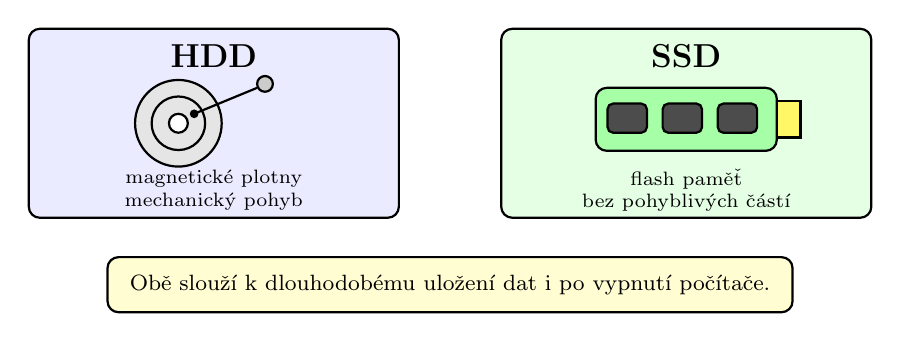
\begin{tikzpicture}[
    x=1cm, y=1cm,
    >=stealth,
    every node/.style={font=\small},
    box/.style={
        draw,
        thick,
        rounded corners,
        align=center
    },
    label/.style={font=\scriptsize, align=center}
]

    % HDD box
    \node[
        box,
        fill=blue!8,
        minimum width=4.7cm,
        minimum height=2.4cm
    ] (hddbox) at (-3.0,0) {};

    \node[font=\large\bfseries] at (-3.0,0.85) {HDD};

    % HDD platter
    \draw[thick, fill=gray!20] (-3.45,0.0) circle (0.55);
    \draw[thick, fill=white] (-3.45,0.0) circle (0.12);
    \draw[thick] (-3.45,0.0) circle (0.34);

    % HDD arm
    \draw[thick] (-2.45,0.45) -- (-3.25,0.12);
    \draw[thick, fill=black] (-3.25,0.12) circle (0.04);
    \draw[thick, fill=gray!40] (-2.35,0.50) circle (0.10);

    \node[label] at (-3.0,-0.85)
        {magnetické plotny\\ mechanický pohyb};

    % SSD box
    \node[
        box,
        fill=green!10,
        minimum width=4.7cm,
        minimum height=2.4cm
    ] (ssdbox) at (3.0,0) {};

    \node[font=\large\bfseries] at (3.0,0.85) {SSD};

    % SSD board
    \draw[thick, rounded corners, fill=green!35]
        (1.85,-0.35) rectangle (4.15,0.45);

    % NAND chips
    \foreach \x in {2.25,2.95,3.65}{
        \draw[thick, rounded corners=2pt, fill=black!70]
            (\x-0.25,-0.12) rectangle (\x+0.25,0.25);
    }

    % Connector
    \draw[thick, fill=yellow!60]
        (4.15,-0.18) rectangle (4.45,0.28);

    \node[label] at (3.0,-0.85)
        {flash paměť\\ bez pohyblivých částí};

    % Comparison note
    \node[
        box,
        fill=yellow!18,
        minimum width=8.7cm,
        minimum height=0.7cm,
        font=\footnotesize
    ] at (0,-2.05)
        {Obě slouží k dlouhodobému uložení dat i po vypnutí počítače.};

\end{tikzpicture}
